\section{Resultados Útiles}

En esta sección pondremos demostraciones que son necesarias o útiles para resolver varios problemas.

\subsection{Argumentos de simetría del campo eléctrico}

Para todas las demostraciones de simetría es necesario tener una distribución uniforme de carga e indicar, inicialmente al menos, de manera gráfica por que existe la simetría. Para cada demostración se hará uso de las coordenadas con la que es más fácil trabajar las figuras, pero aplica para todas las coordenadas haciendo las transformaciones pertinentes.

\subsubsection{En esferas}

\label{SimetríaEsfera}
En esferas el campo eléctrico tiene componente solo en $\hat{r}$ a causa de que los campos generados por cargas cercanas se cancelan entre sí, permitiendo solo la existencia en esa dirección. 

En la figura inferior se observa que los campos $\Vec{E}_2$ y $\Vec{E}_1$ generados por $\Delta q_1$ y $\Delta q_2$ en la dirección $P$ se cancelan entre sí, causando el campo $\Vec{E}_{neto}$ en la dirección radial a $P$.
\begin{figure}[H]
    \centering
    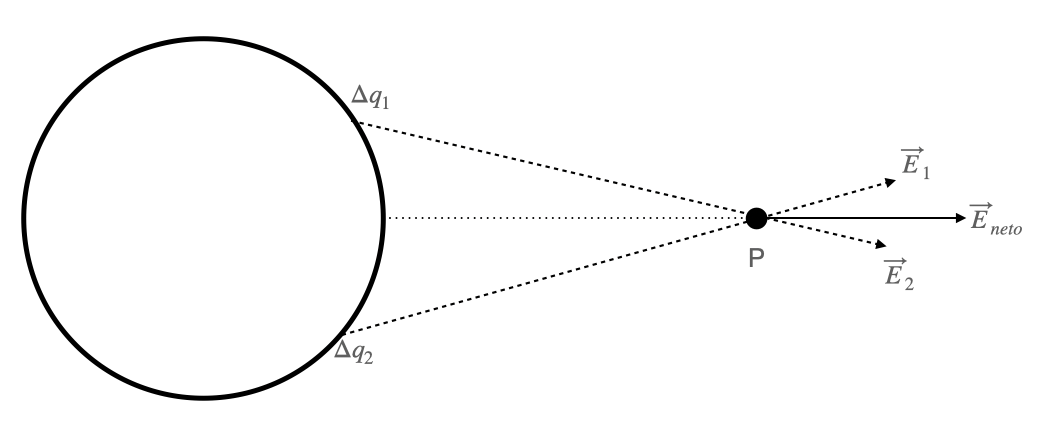
\includegraphics[width=0.7\textwidth]{Resultados utiles/demost_simetria_esfera.png}
    \label{fig:simetria_esfera}
\end{figure}

\subsubsection{En cilindros infinitos o con altura $\gg$ radio}

\label{SimetríaCilindrosInf}
En cilindros tales que sean de largo infinito o su largo sea mucho mayor ($\gg$) al radio, el campo eléctrico apuntará en la dirección $\hat{\rho}$, esto a que las componentes de los campos en $\hat{z}$ se cancelan entre sí.

En la figura inferior se observa esto, donde en el punto $P$ los campos $\Vec{E}_1$ y $\Vec{E}_2$ generados por $\Delta q_1$ y $\Delta q_2$ se cancelan entre sí dando origen al campo $\Vec{E}_{neto}$ en $\hat{\rho}$.
\begin{figure}[H]
    \centering
    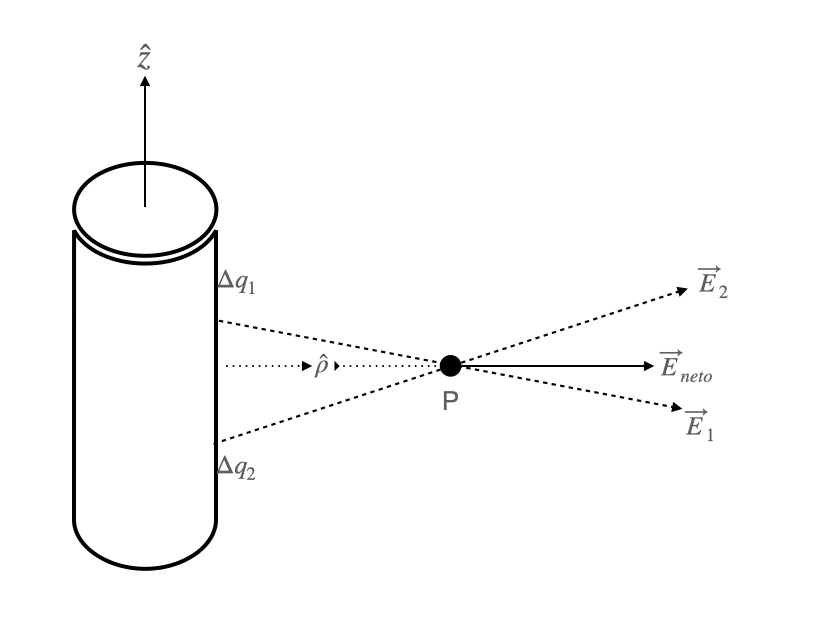
\includegraphics[width=0.7\textwidth]{Resultados utiles/demost_simetria_cili.png}
    \label{fig:simetria_cilindro}
\end{figure}
\subsubsection{En planos infinitos}
\label{SimetríaPlanosInf}
En planos infinitos o con largo 'muy grande', se tendrá que el campo solo apuntará en la dirección normal a la superficie, esto es a causa de que las componentes en las otras direcciones se cancelan entre sí. 
\medbreak
En la figura inferior se observa esto, donde la normal es $\hat{z}$.
\begin{figure}[H]
    \centering
    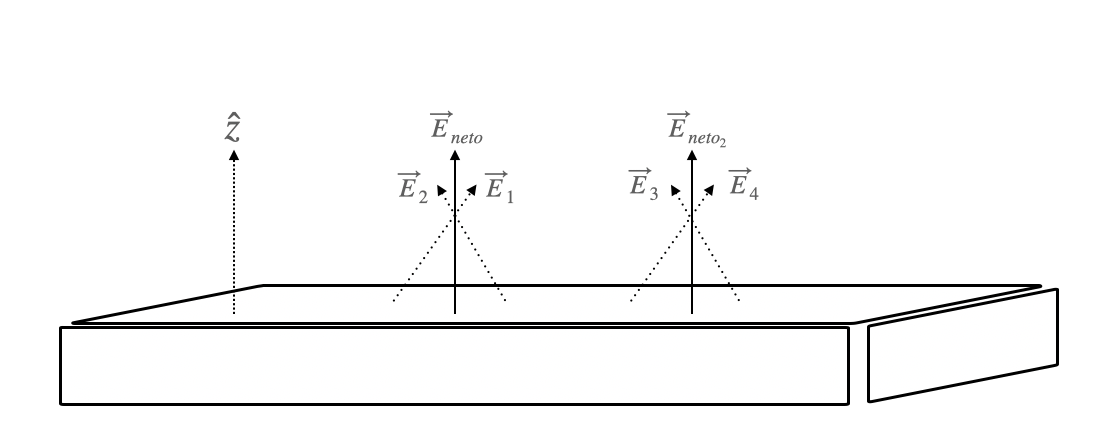
\includegraphics[width=0.7\textwidth]{Resultados utiles/demost_simetria_plano.png}
    \label{fig:simetria_plano}
\end{figure}
\medbreak
Tomando un punto $r$ arbitrario fuera del plano en el lado donde $z$ es positivo, para todo punto $p$ en el plano, existe $p'$ simétrico a $p$ respecto a la recta perpendicular al plano que pasa por $r$, tal que la suma de los vectores que apuntan de $p$ a $r$ y de $p'$ a $r$ es paralela al eje $z$

\[\Vec{pr} = \Vec{r}-\Vec{p} = (r_x-p_x)\hat{x} + (r_y-p_y)\hat{y} + r_z\hat{z}\]
\[\Vec{p'r} = \Vec{r}-\Vec{p'} = (p_x-r_x)\hat{x} + (p_y-r_y)\hat{y} + r_z\hat{z}\]
\[\Vec{pr}+\Vec{p'r} = 2r_z\hat{z}\]

Con esto, el campo eléctrico en el lado positivo de $z$ depende sólo de $z$

\[\Vec{E_p}(\Vec{z})=E_p(z)\hat{z}\]

El razonamiento es el mismo para el lado negativo de z, con la única diferencia que el campo apunta en sentido opuesto.

\subsection{Ecuación de Poisson para esferas}
\label{PoissonEsferas}
Por simetría el potencial de una esfera depende sólo de la componente $r$ de las coordenadas esféricas.


\[\nabla^2V =
\nabla\cdot\left(\frac{\partial V}{\partial r}\hat{r}\right) =
\frac{1}{r^2}\frac{\partial}{\partial r}\left(\frac{\partial V}{\partial r}r^2\right) =
\frac{\partial^2 V}{\partial r^2}+\frac{2}{r}\frac{\partial V}{\partial r}
\]
\begin{equation}
\begin{split}
\nabla^2V = -\frac{\rho}{\epsilon_o} & \Leftrightarrow
\frac{\partial}{\partial r}\left(\frac{\partial V}{\partial r}r^2\right) = -\frac{\rho r^2}{\epsilon_o}
\\
& \Leftrightarrow \frac{\partial V}{\partial r}r^2 =
-\frac{\rho}{\epsilon_o}\int r^2\,dr
\\
& \Leftrightarrow \frac{\partial V}{\partial r} =
\frac{A}{r^2} - \frac{\rho r}{3\epsilon_o}
\\
& \Leftrightarrow V =
\int\frac{A}{r^2} - \frac{\rho r}{3\epsilon_o}\,dr
\\
& \Leftrightarrow V = 
B-\frac{A}{r} - \frac{\rho r^2}{6\epsilon_o}
\\
\end{split}
\nonumber
\end{equation}

\subsection{Ecuación de Poisson para cilindros infinitos}
\label{PoissonCilindrosInf}
Por simetría el potencial de una cilindro infinito depende sólo de la componente $\rho$ de las coordenadas cilíndricas, la cual notaremos como $r$ para distinguirla de la densidad de carga volumétrica.

\[\nabla^2V =
\nabla\cdot\left(\frac{\partial V}{\partial r}\hat{r}\right) =
\frac{1}{r}\frac{\partial}{\partial r}\left(\frac{\partial V}{\partial r}r\right) =
\frac{\partial^2 V}{\partial r^2}+\frac{1}{r}\frac{\partial V}{\partial r}
\]

\begin{equation}
\begin{split}
\nabla^2V = -\frac{\rho}{\epsilon_o} & \Leftrightarrow
\frac{\partial}{\partial r}\left(\frac{\partial V}{\partial r}r\right) = -\frac{\rho r}{\epsilon_o}
\\
& \Leftrightarrow \frac{\partial V}{\partial r}r =
-\frac{\rho}{\epsilon_o}\int r\,dr
\\
& \Leftrightarrow \frac{\partial V}{\partial r} =
\frac{A}{r} - \frac{\rho r}{2\epsilon_o}
\\
& \Leftrightarrow V =
\int\frac{A}{r} - \frac{\rho r}{2\epsilon_o}\,dr
\\
& \Leftrightarrow V = 
A\ln{r} - \frac{\rho r^2}{4\epsilon_o} + B
\\
\end{split}
\nonumber
\end{equation}

\subsection{Capacitancia de placas cercanas}
\label{C:placas}
Para el caso de un condensador conformado por 2 placas geométricamente idénticas de área $A$ separadas por una distancia $d$, si $d$ es mucho menor a las dimensiones de las placas se puede aproximar el campo eléctrico al de una placa infinita (2 planos infinitos), este está dado por

\[\Vec{E}=\frac{\sigma}{\epsilon_o}\]

donde $\sigma$ es la densidad de carga de una de las placas. De la relación\newline $\Vec{E}=-\nabla V$ se desprende que el potencial entre las placas es

\[V(z) = -\frac{\sigma z}{\epsilon_o}+B\]

con $B$ una constante. La diferencia de potencial del condensador es

\[\Delta V=V(0)-V(d)=B-
\left(-\frac{\sigma d}{\epsilon_o}+B\right) =
\frac{\sigma d}{\epsilon_o}\]

finalmente, se obtiene la capacitancia como

\[C=\frac{Q}{\Delta V}=\frac{\epsilon_o}{\sigma d}\sigma A=
\frac{\epsilon_o A}{d}\]

\subsection{Índice de Soluciones}

\begin{itemize}
    \item $\Vec{E}$ de un plano infinito: \hyperlink{S.4.2}{\textbf{S.4.2}} c)
    \item $U_e$ de un cascarón esférico: \hyperlink{S.6.1}{\textbf{S.6.1}}
    \item Fuerza, torque y energía en relación al momento dipolar: \hyperlink{S.8.1}{\textbf{S.8.1}}
\end{itemize}

\newpage